\chapter{Estudo de caso}\label{estudo_de_caso}

A metodologia desenvolvida no decorrer desse trabalho foi aplicada a um banco de dados real, proveniente de uma grande mineradora de ouro. Para verificar a competência do método, o modelo criado implicitamente pelo algoritmo proposto foi comparado com um modelo criado por um geomodelador, através da digitalização manual de polígonos em seções, e posterior construção dos sólidos que representam as unidades litológicas. Assim, foi possível avaliar se as estruturas geológicas interpretadas foram satisfatoriamente reproduzidas pelo algoritmo.

O banco de dados categóricos fornecido abrange 9140 amostras, distribuídas entre cinco diferentes litologias. O depósito cobre uma área de aproximadamente $10km^2$ com $1300m$ de profundidade. Maiores detalhes em relação à geologia e localização do depósito serão omitidos por questões de confidencialidade.

A \autoref{dados} evidencia as amostras em planta, à esquerda, e em perfil, à direita. Enquanto a \autoref{dados_hist}, mostra o histograma dos dados, que expressa as proporções de cada litologia nos dados amostrais.

\begin{figure}[H]
	\caption{\label{dados}Dados em planta à esquerda e em perfil à direita.}
	\begin{center}
		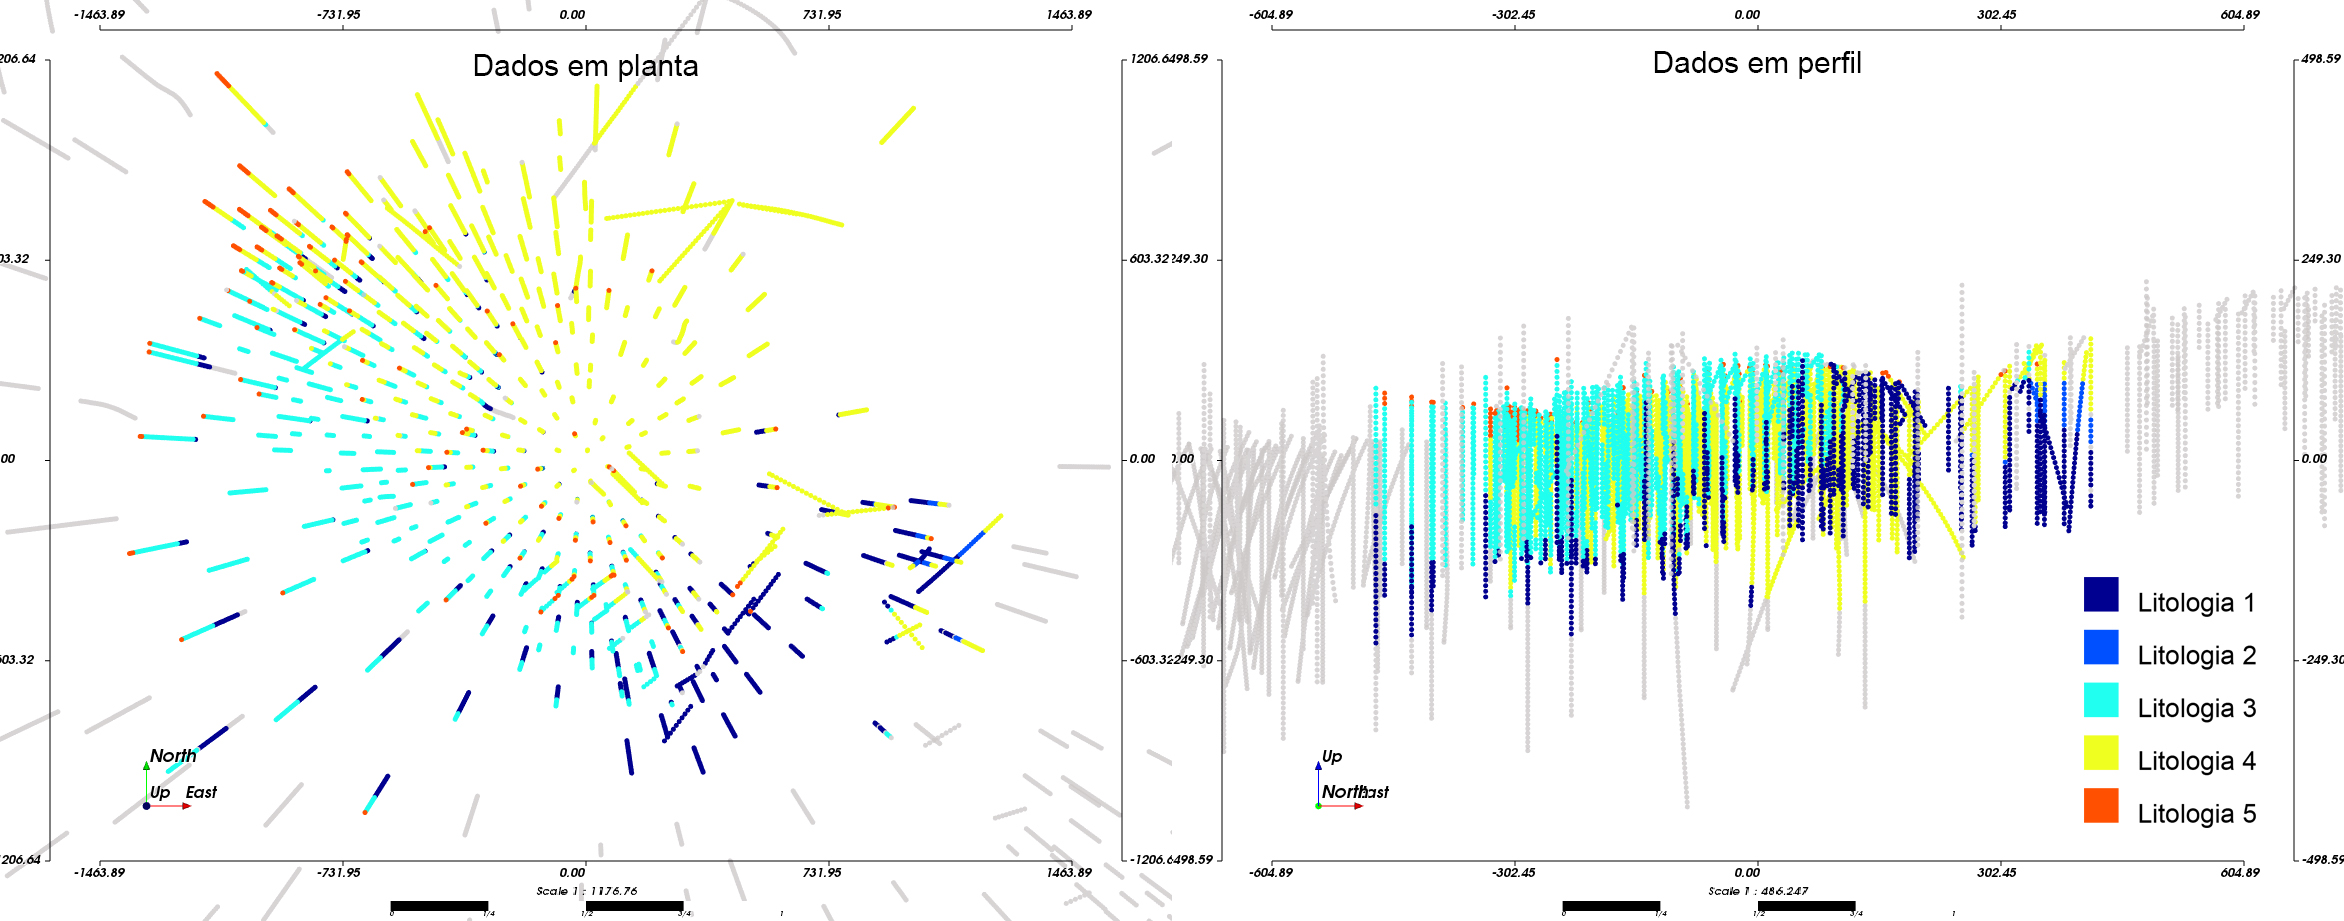
\includegraphics[width=\textwidth]{estudo_de_caso/dados}
	\end{center}
	%\legend{Fonte: Modificado de \citeonline{maureira}}
\end{figure}

\begin{figure}[!htb]
	\caption{\label{dados_hist}Histograma dos dados.}
	\begin{center}
		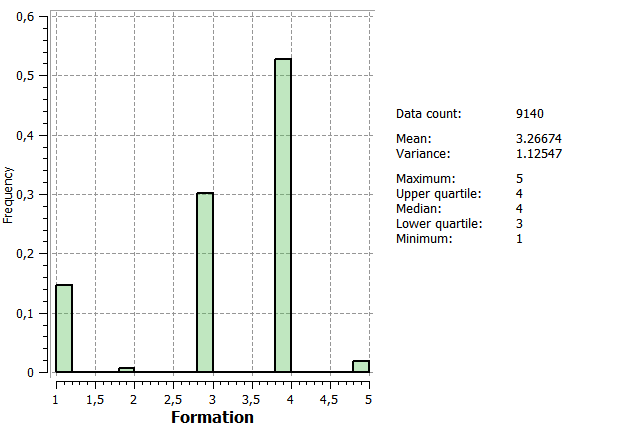
\includegraphics[width=0.5\textwidth]{estudo_de_caso/histograma_dados}
	\end{center}
	%\legend{Fonte: Modificado de \citeonline{maureira}}
\end{figure}

A partir das amostras, o valor da função distância assinalada foi calculado para cada litologia, em cada ponto amostral. O depósito não apresenta morfologia que justifique o cálculo de distâncias anisotrópicas, então, o caso isotrópico foi escolhido.

A \autoref{signed_distances_estudo} mostra as distâncias assinaladas calculadas para cada uma das cinco litologias, a transição suave entre as cores denota o comportamento extremamente contínuo das distâncias assinaladas.

\begin{figure}[H]
	\caption{\label{signed_distances_estudo}Distâncias assinaladas calculadas para cada uma das litologias.}
	\begin{center}
		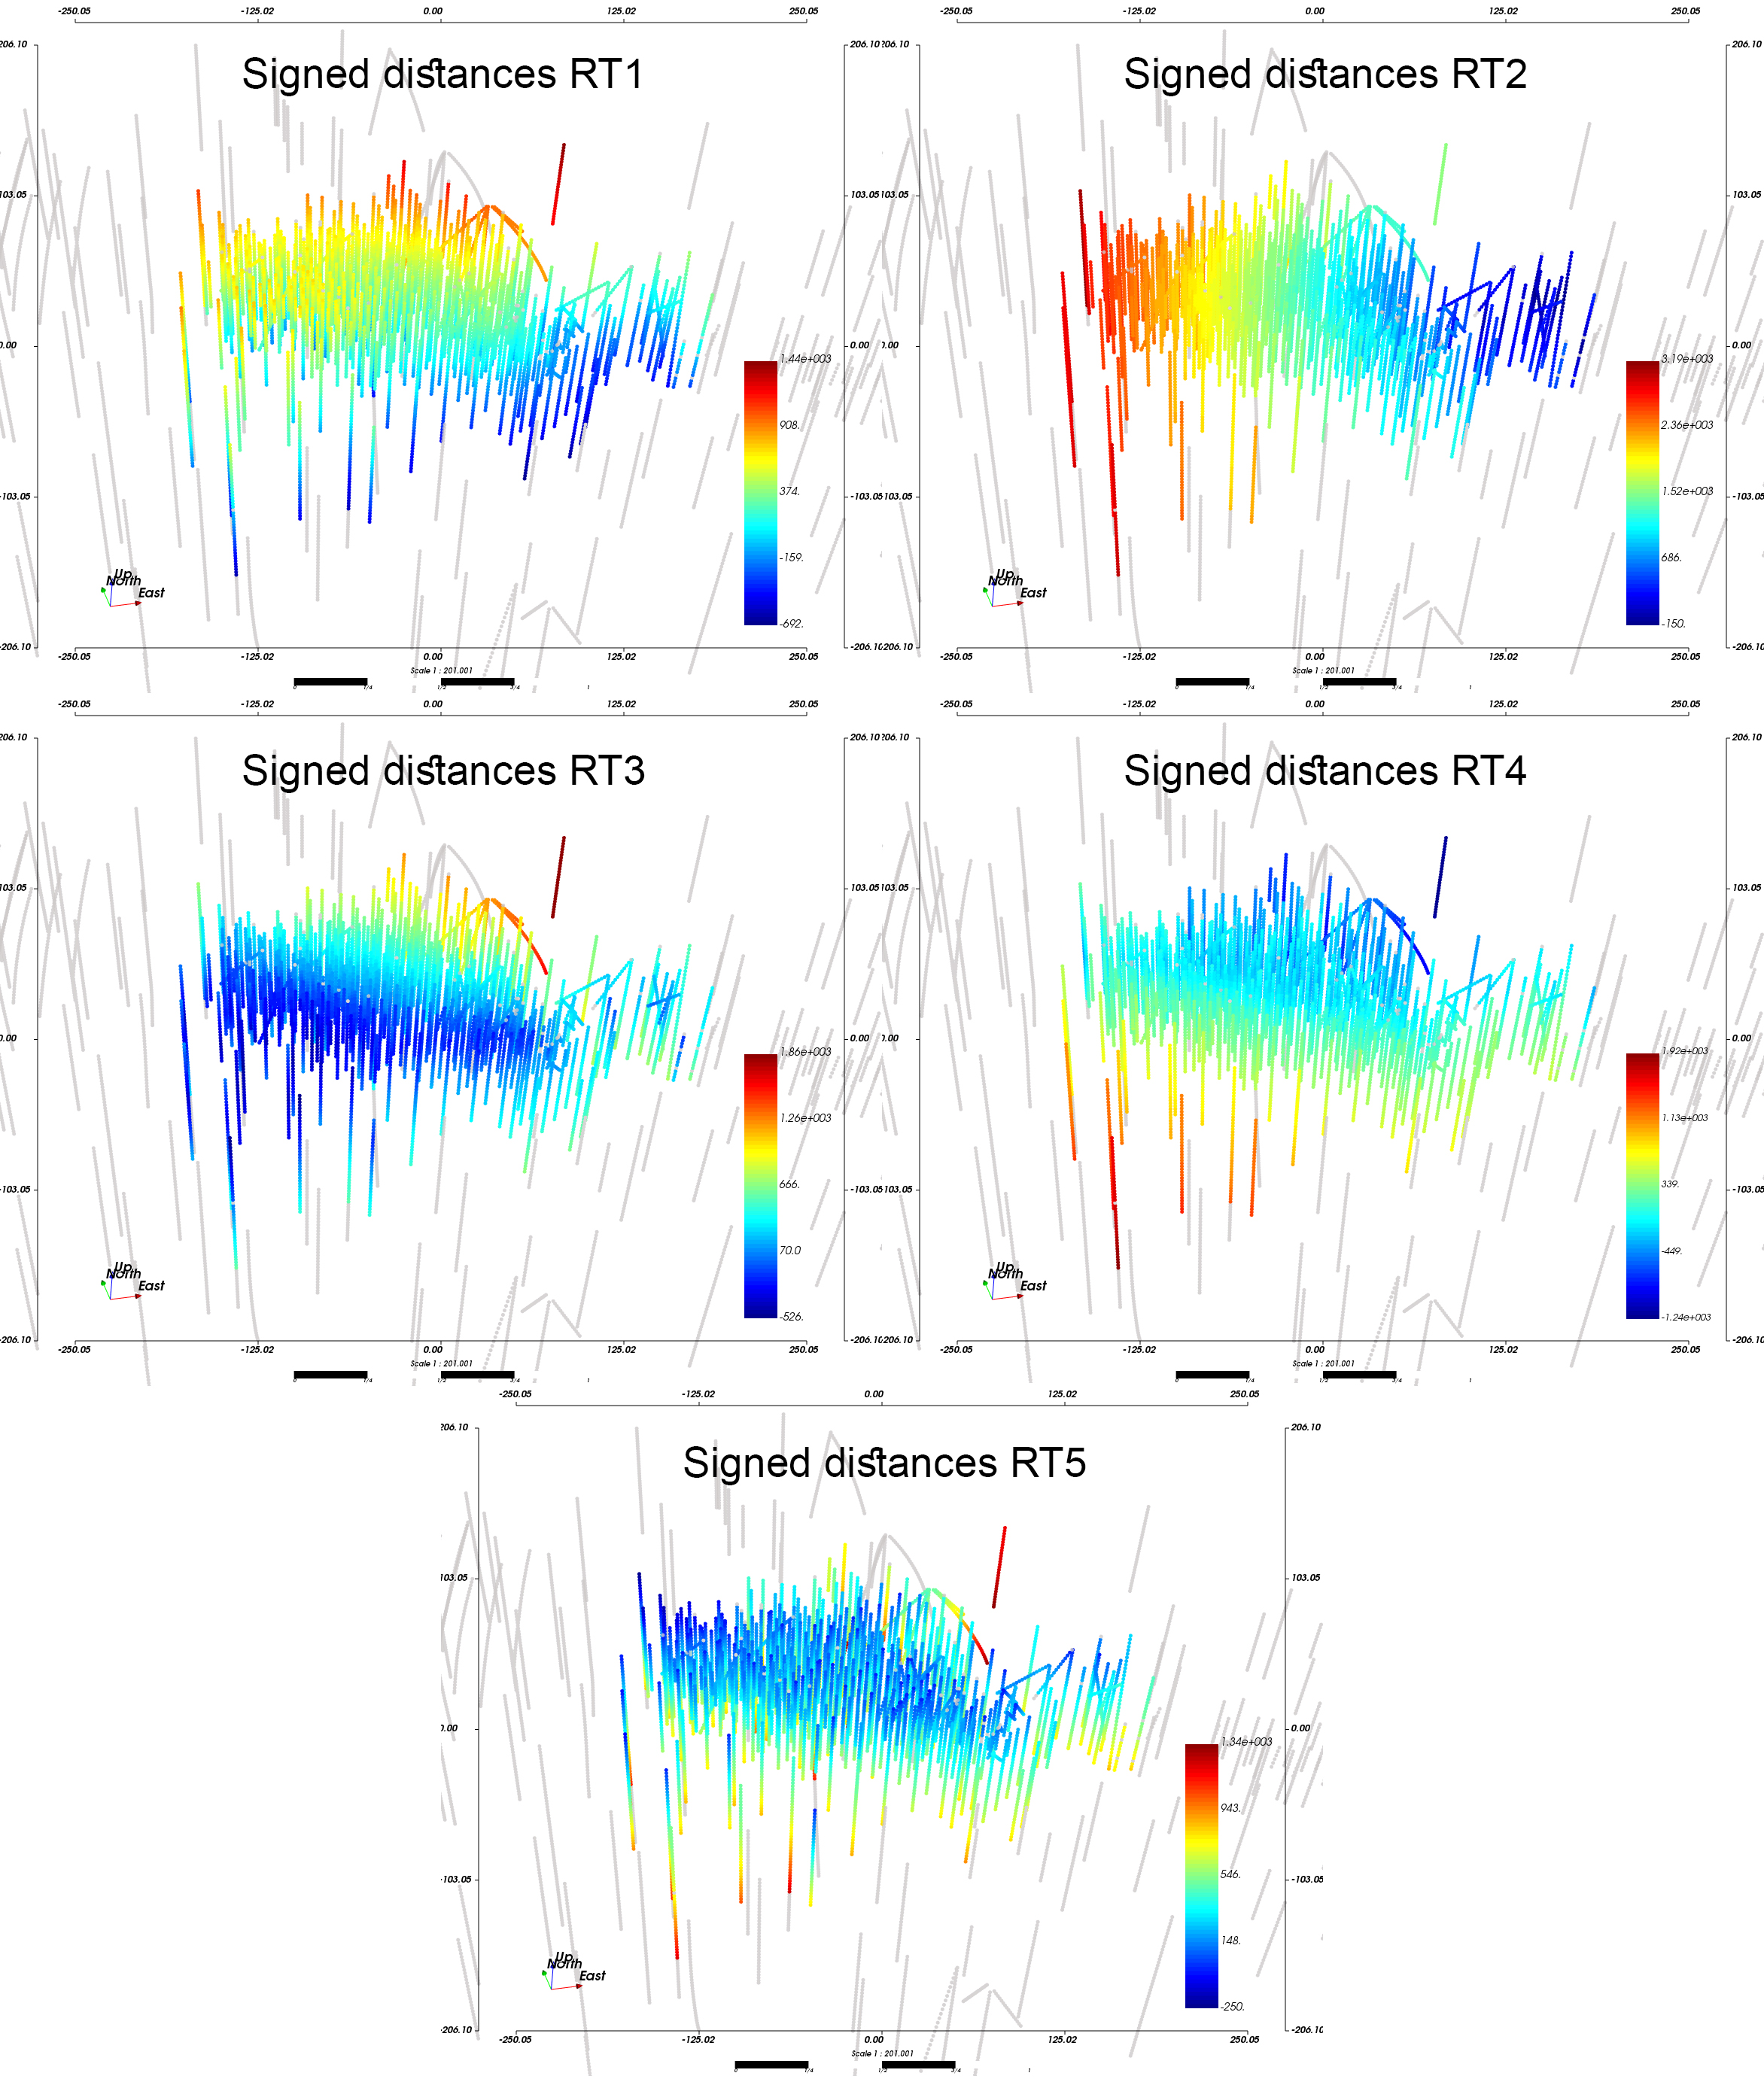
\includegraphics[width=0.9\textwidth]{estudo_de_caso/signed_distances}
	\end{center}
	%\legend{Fonte: Modificado de \citeonline{maureira}}
\end{figure}

\section{Variografia}

As distâncias assinaladas apresentam, além do comportamento extremamente contínuo observado na \autoref{signed_distances_estudo}, um comportamento não estacionário. Isto é, seu variograma experimental não se estabiliza em um patamar. Essa característica torna a inferência do alcance arbitrária, como observado na \autoref{variogramas}. 

O alcance do variograma, juntamente com a anisotropia, controlam a extensão e forma dos domínios modelados. Na \autoref{analise_range}, a litologia 1 foi modelada a partir de três valores diferentes de alcance de um variograma isotrópico, mantido o mesmo patamar: 150m à esquerda, 1500m no centro, e 15000m à direita. O variograma das demais litologias não foi alterado.

Ao aumentar o alcance do variograma de um dos domínios modelados, a estrutura associada à esse domínio ganha um corpo mais volumoso, crescendo na direção de maior continuidade do variograma, e consequentemente sua proporção no depósito aumenta, como observado na análise da litologia 1 da \autoref{analise_range}. A diferença entre as proporções não é muito pronunciada já que a densidade amostral do banco de dados é muito alta. Em análise semelhante, \citeonline{maureira} obteve resultados análogos.  

A inferência do alcance dos variogramas pode se tornar arbitrária devido ao comportamento não estacionário das distâncias assinaladas. Uma alternativa consiste em fixar a variância dos variogramas na variância \textit{a priori} dos dados, e ajustar um modelo ao variograma experimental dessa forma. Uma outra alternativa é inferir o alcance a partir das dimensões das estruturas observadas nos dados amostrais.

\begin{figure}[H]
	\caption{\label{analise_range}Litologia 1, e respectiva proporção, modelada variando o range do variograma: $150m$ à esquerda, $1500m$ ao centro e $15000m$ à direita.}
	\begin{center}
		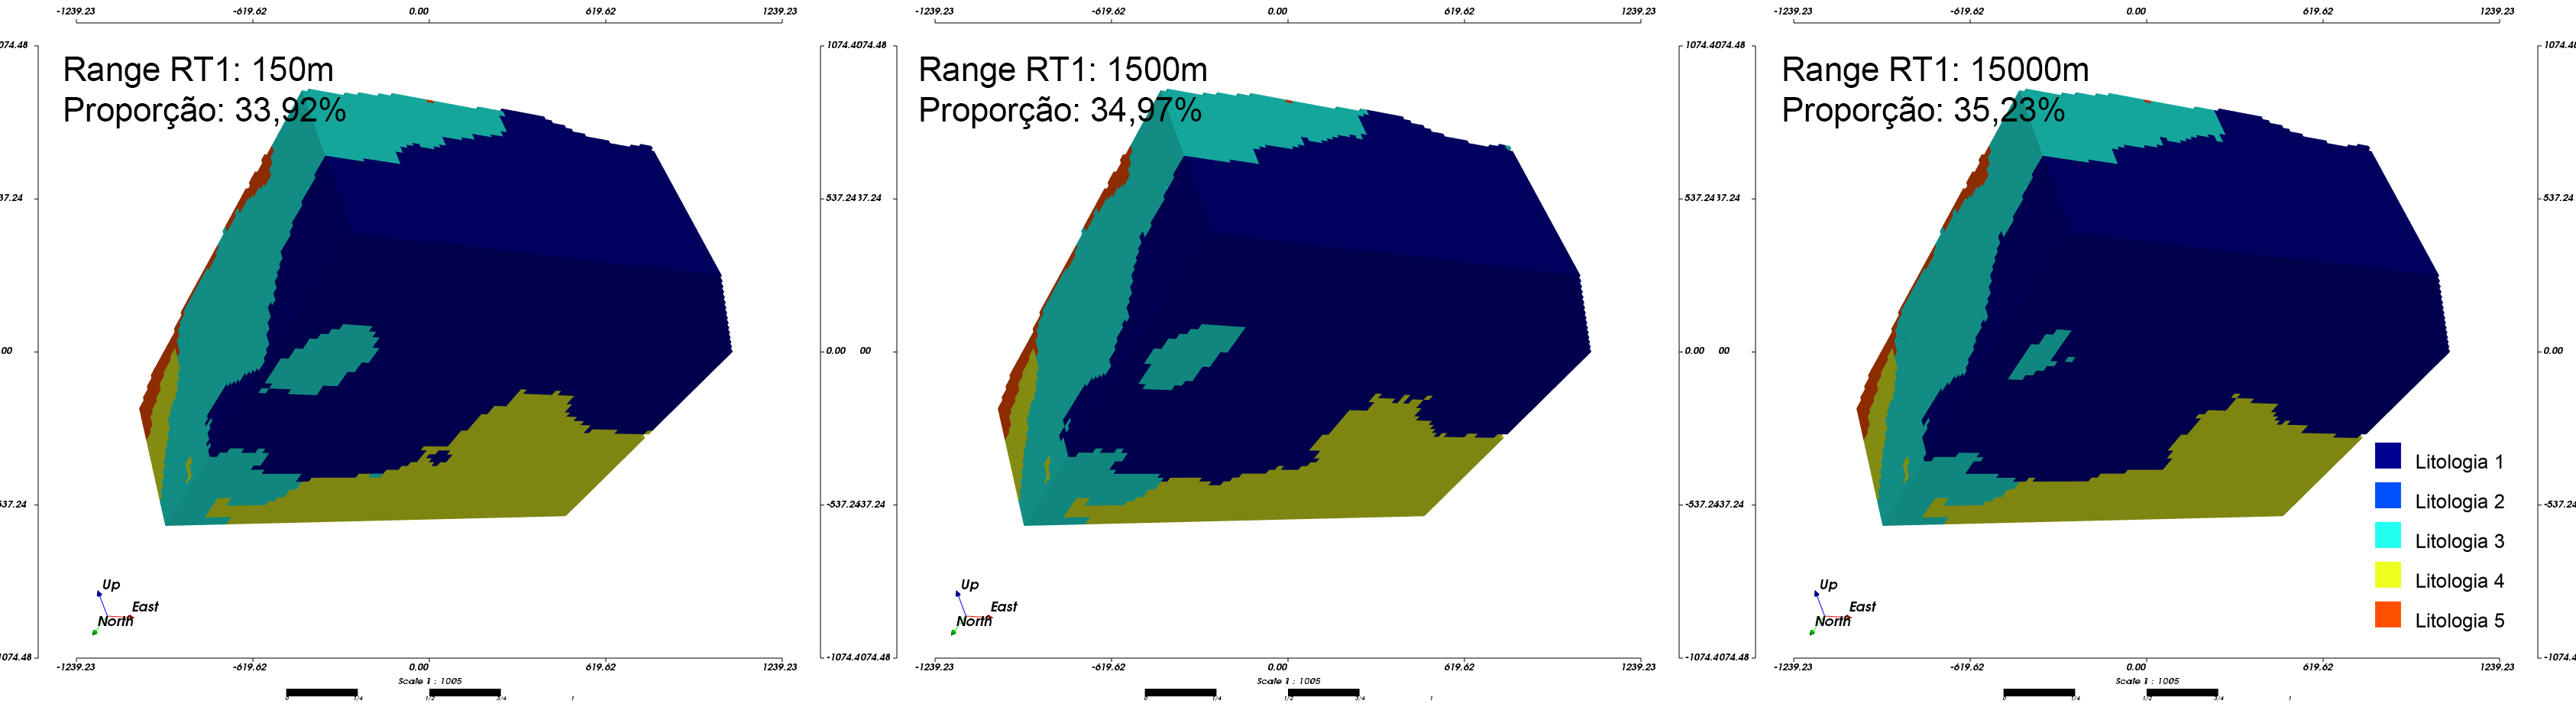
\includegraphics[width=\textwidth]{estudo_de_caso/analise_range}
	\end{center}
	%\legend{Fonte: Modificado de \citeonline{maureira}}
\end{figure}

Os variogramas experimentais das distâncias assinaladas nunca exibem efeito pepita. Porém, este pode ser adicionado arbitrariamente pelo usuário para controlar a interconectividade dos domínios. A \autoref{analise_efeito_pepita} mostra quatro modelos gerados a partir de variogramas isotrópicos com o mesmo alcance para todas as litologias e seus respectivos histogramas. Apenas a proporção entre a contribuição do efeito pepita e a contribuição total do variograma foi alterada, da mesma maneira, para todas as litologias.

Na \autoref{analise_efeito_pepita}, da esquerda para a direita, não há efeito pepita algum na primeira imagem, 10\% de efeito pepita na segunda imagem, 50\% e 90\% de efeito pepita nas imagens seguintes.

\begin{figure}[!htb]
	\caption{\label{analise_efeito_pepita}Modelos calculados a partir de variogramas com diferentes proporções de efeito pepita. Da direita para a esquerda: 0\%, 10\%, 50\% e 90\%.}
	\begin{center}
		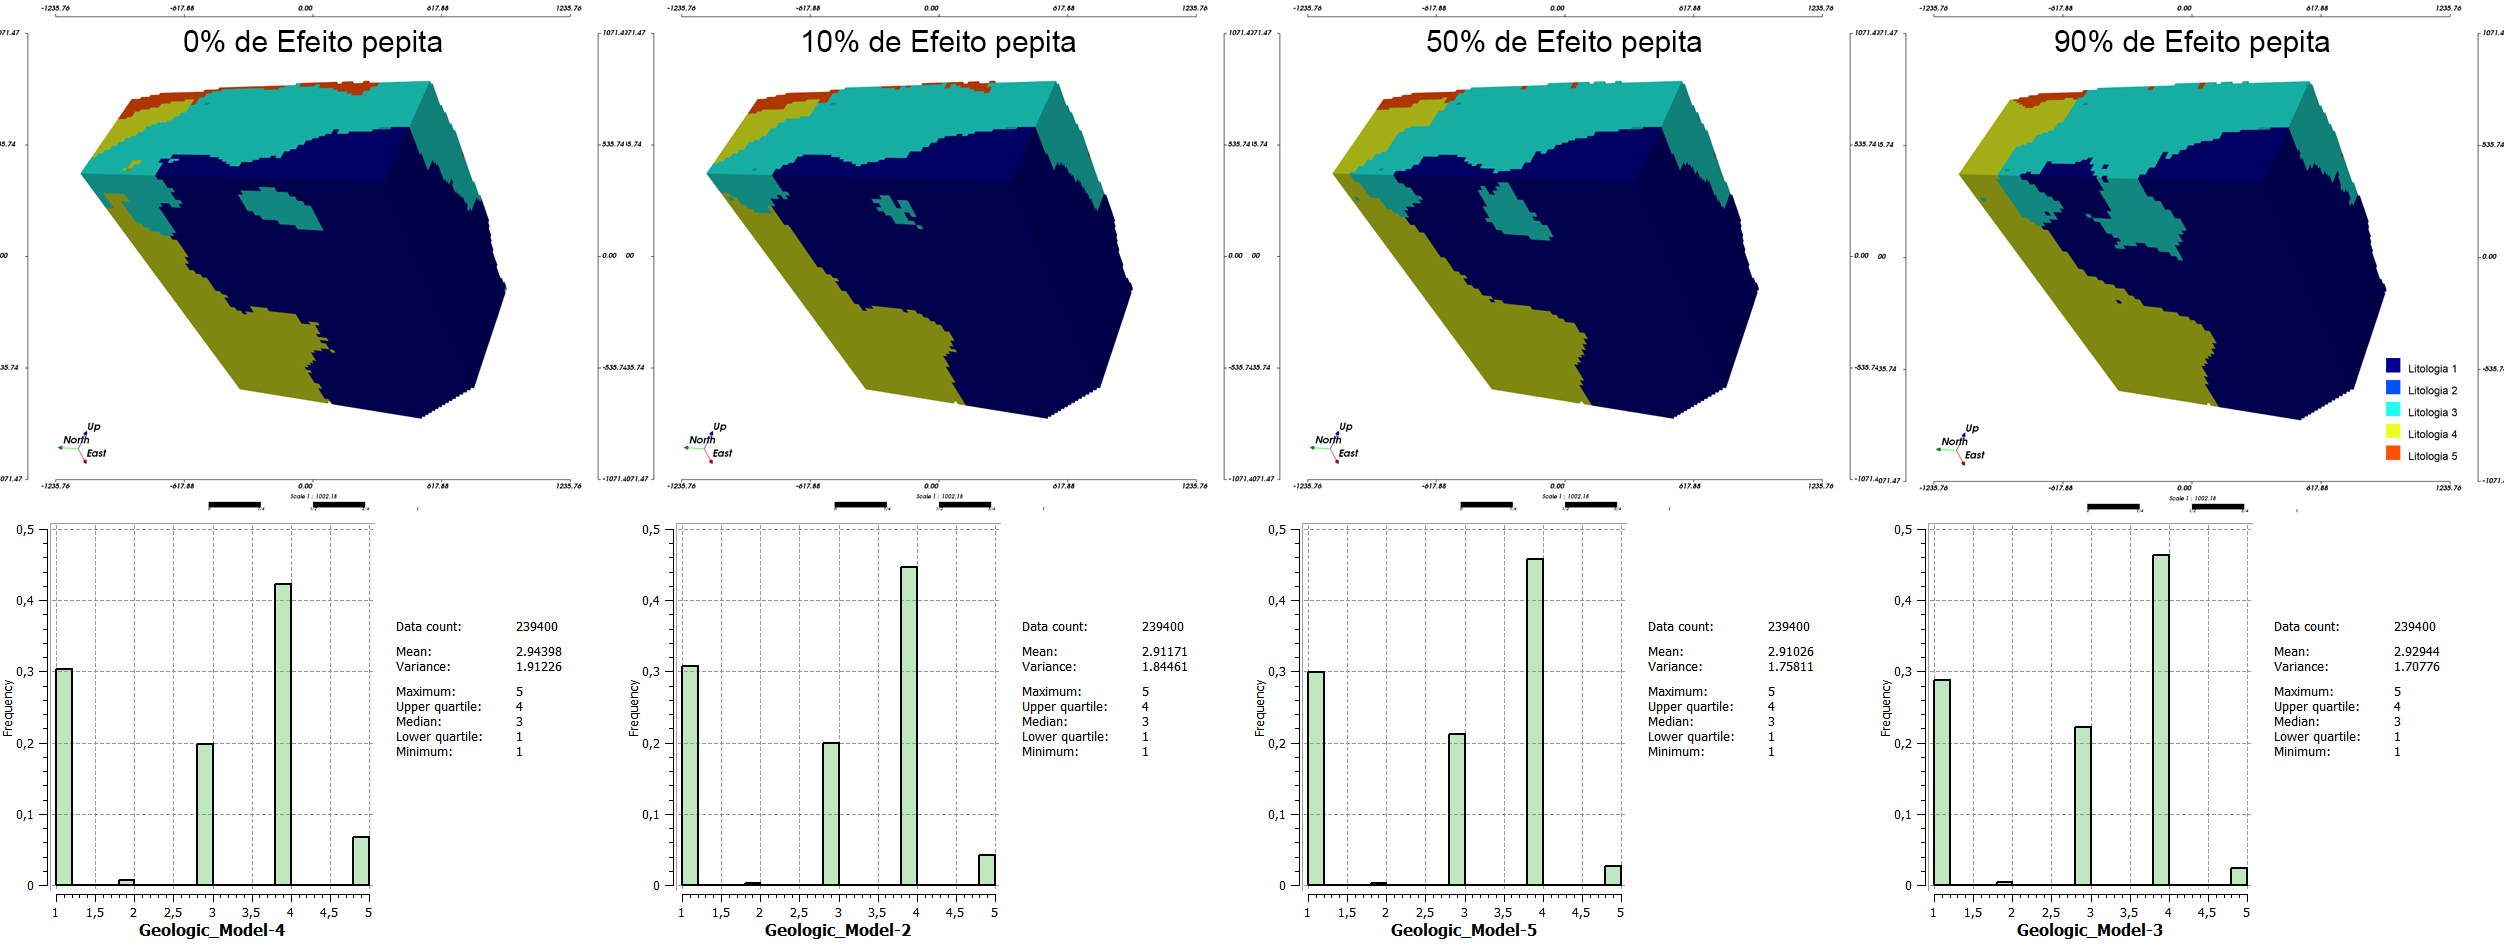
\includegraphics[width=\textwidth]{estudo_de_caso/efeito_pepita}
	\end{center}
	%\legend{Fonte: Modificado de \citeonline{maureira}}
\end{figure}

O efeito do aumento da contribuição do efeito pepita para a variância total é mais pronunciado na litologia 1, é possível observar que a medida que a contribuição aumenta o domínio representado pela litologia 1 se torna mais desconexo. Na última imagem (90\% de efeito pepita), pode-se observar dois "braços" que são interligados quando o modelo é gerado com proporções menores de efeito pepita nos variogramas. Os histogramas pouco se alteram, novamente, devido à alta densidade amostral do banco de dados.

Posto isso, os variogramas experimentais das distâncias assinaladas referentes às cinco litologias do depósito foram calculados, a partir dos parâmetros da \autoref{param_var}, e modelados. Os variogramas não apresentaram nenhuma direção preferencial de continuidade. A \autoref{variogramas} mostra os variogramas experimentais isotrópicos para todas as cinco distâncias assinaladas e seu respectivo modelo ajustado (\autoref{varsd1} a \autoref{varsd5}).

\begin{table}[!ht]
\centering
\caption{Parâmetros para o cálculo da variograma experimental.}
\label{param_var}
\begin{tabular}{cccc}
nº de lags & sep. lag (m) & tol. lag (m) & larg. de banda (m) \\ \hline
20         & 100      & 50       & 50             \\ \hline
\end{tabular}
\end{table}

O comportamento contínuo das distâncias faz com que o modelo gaussiano seja o que melhor se ajusta aos pontos do variograma experimental, geralmente, apenas uma estrutura é suficiente para um bom ajuste. O efeito pepita foi adicionado arbitrariamente para controlar a interconexão entre as litologias.

\begin{figure}[!htb]
	\caption{\label{variogramas} Variograma das distâncias assinaladas calculadas para cada uma das litologias.}
	\begin{center}
		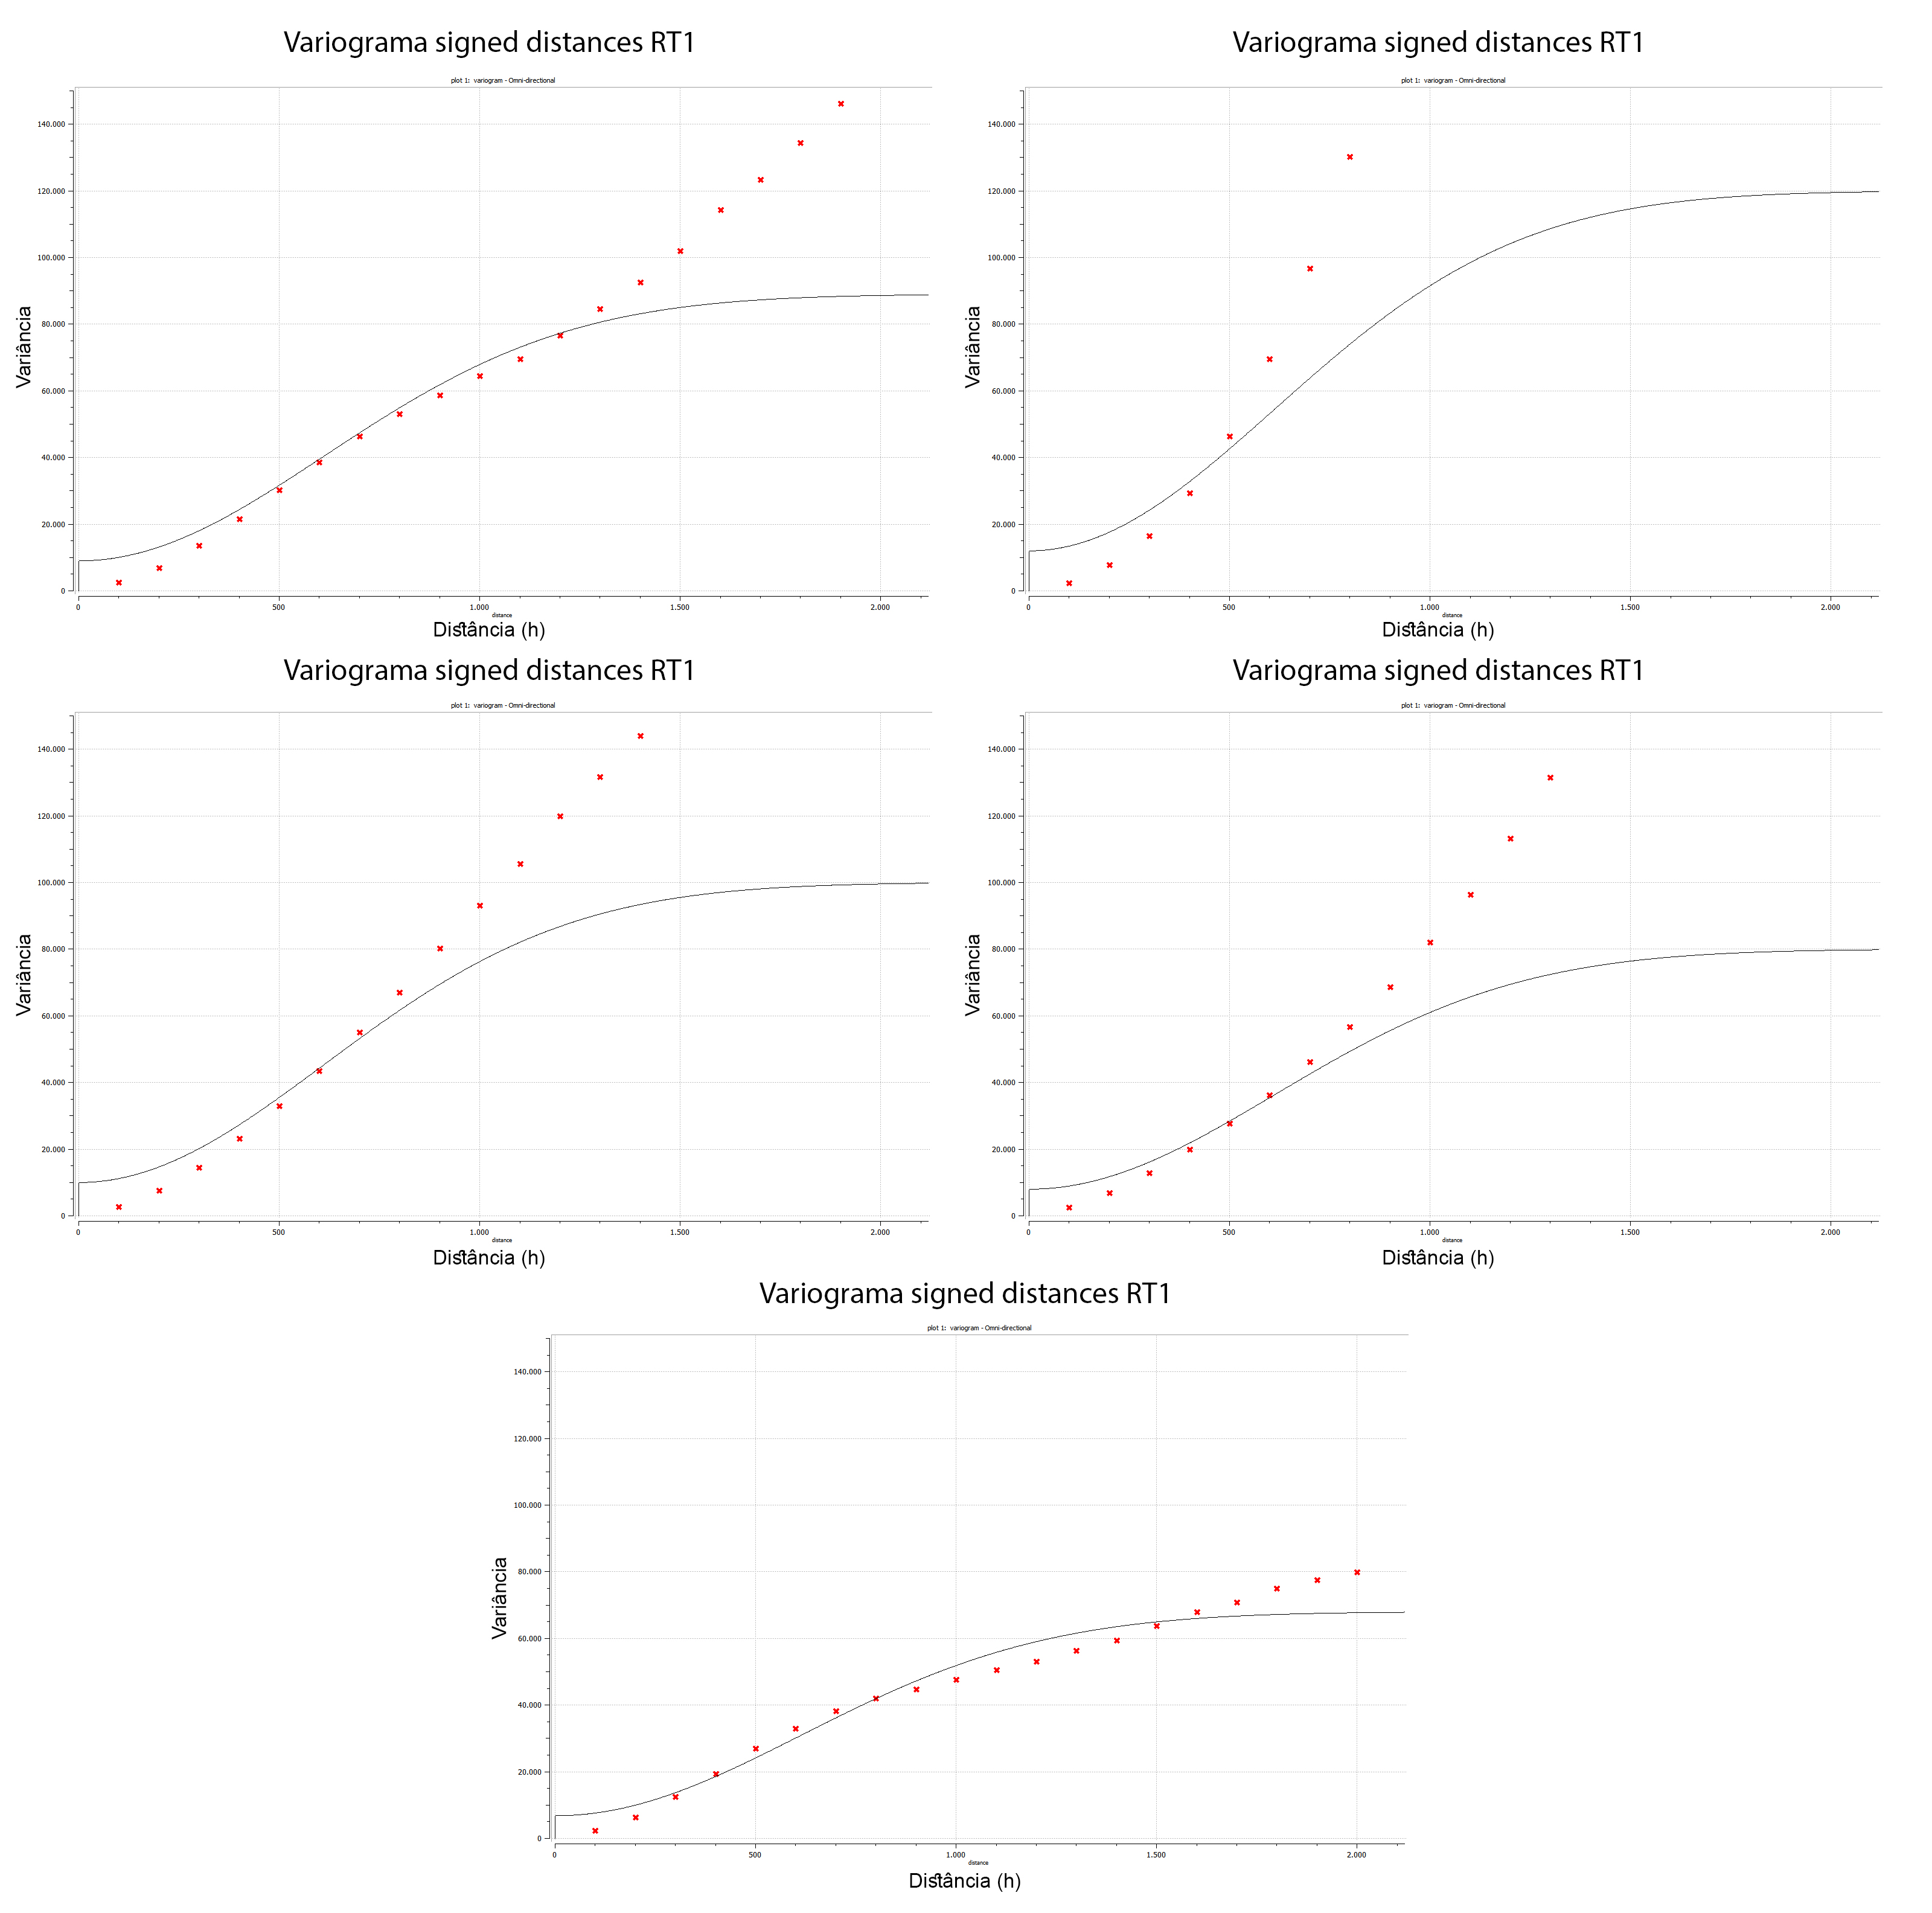
\includegraphics[width=\textwidth]{estudo_de_caso/var}
	\end{center}
	%\legend{Fonte: Modificado de \citeonline{maureira}}
\end{figure}

\begin{equation}
\label{varsd1}
\gamma_{SD1}(h)=9000+80000gauss\left(\frac{h}{1500m}\right)
\end{equation}

\begin{equation}
\label{varsd2}
\gamma_{SD2}(h)=12000+108000 gauss\left(\frac{h}{1500m}\right)
\end{equation}

\begin{equation}
\label{varsd3}
\gamma_{SD3}(h)=10000 +90000 gauss\left(\frac{h}{1500m}\right)
\end{equation}

\begin{equation}
\label{varsd4}
\gamma_{SD4}(h)=8000  +72000  gauss\left(\frac{h}{1500m}\right)
\end{equation}

\begin{equation}
\label{varsd5}
\gamma_{SD5}(h)=6800   +61200   gauss\left(\frac{h}{1500m}\right)
\end{equation}

O valor absoluto da variância dos variogramas não tem influência alguma no resultado da krigagem ordinária, somente na variância de krigagem, que não é usada para criar os modelos gerados implicitamente pelo método das distâncias assinaladas. Apenas a proporção das contribuições das estruturas para a variância total modifica o resultado da krigagem. Como os modelos ajustados aos variogramas experimentais da \autoref{variogramas} apresentam, todos eles, proporção de 10\% efeito pepita e 90\% de contribuição da estrutura gaussiana, além do mesmo range, foi possível o uso do mesmo modelo variográfico da \autoref{var} para todas as litologias.

\begin{equation}
\label{var}
\gamma_{SD}(h)=0,1+0,9gauss\left(\frac{h}{1500m}\right)
\end{equation}

\section{Interpolação}

As distâncias calculadas e posteriormente variografadas, foram interpoladas no mesmo \textit{grid} do modelo de referência fornecido. As propriedades do \textit{grid} são mostradas na \autoref{Grid_Parameters}. Uma máscara (\textit{region}) correspondente à topografia foi aplicada à esse \textit{grid}.  

\begin{table}[!htb]
\centering
\caption{Propriedades do \textit{grid}.}
\label{Grid_Parameters}
%\begin{adjustbox}{width=0.7\textwidth}
\begin{tabular}{cccccc}
\multicolumn{3}{c}{Número de blocos} & \multicolumn{3}{c}{Dimensão dos blocos (m)} \\ \hline
Num. X     & Num. Y     & Num. Z     & Dim. X     & Dim. Y     & Dim. Z     \\
70         & 60         & 57         & 50        & 50        & 25        \\ \hline
\end{tabular}
%\end{adjustbox}
\end{table}

As distâncias foram interpoladas por krigagem ordinária em todos os nós do \textit{grid}, com a estratégia de krigagem da \autoref{Kriging_parameter}.  

\begin{table}[!htb]
\centering
\caption{Parâmetros de krigagem ordinária.}
\label{Kriging_parameter}
%\begin{adjustbox}{width=0.7\textwidth}
\begin{tabular}{cccccc}
                & \multicolumn{3}{c}{Vizinhança de busca (m)}     & \multicolumn{2}{c}{Número de amostras} \\ \hline
                & Raio (X) & Raio (Y) & Raio (Z) & Min. amostras      & Max. amostras      \\
Litologias (1-5) & 3000      & 3000      & 3000      & 4                 & 40                \\ \hline
\end{tabular}
%\end{adjustbox}
\end{table}

A \autoref{num_amostras} mostra, à esquerda, um scatterplot categórico entre um modelo criado utilizando no máximo 40 amostras por estimativa, no eixo x, e no eixo y, um modelo criado usando no máximo 100 amostras por estimativa. E à direita, um outro \textit{scatterplot,} o mesmo modelo criado utilizando no máximo 40 amostras, no eixo x, e no eixo y, um modelo criado usando no máximo 200 amostras por estimativa. Todas as estratégias de krigagem utilizadas apresentam alcance de busca suficientemente grande para abranger o número máximo de amostras.

\begin{figure}[H]
	\caption{\label{num_amostras}Scatterplots entre modelos gerados com diferentes estratégias de krigagem.}
	\begin{center}
		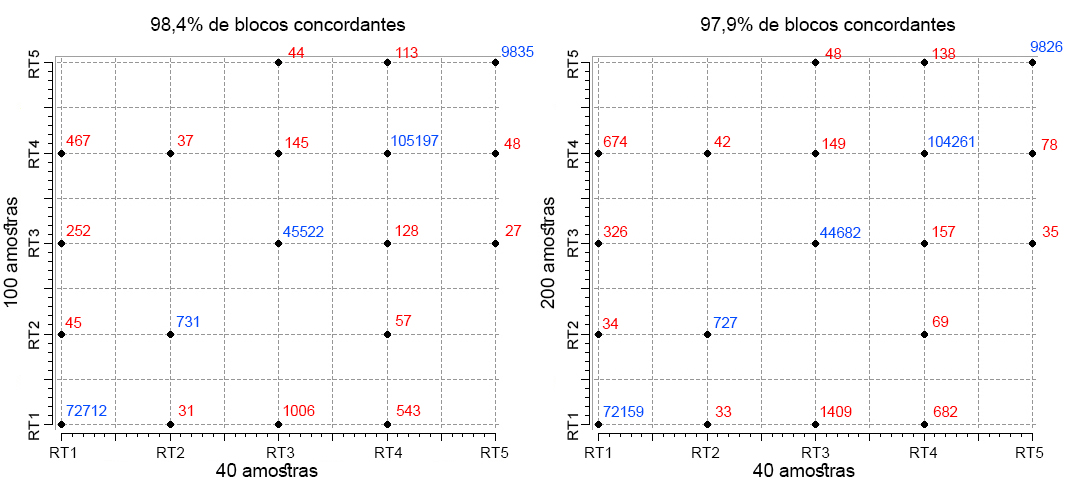
\includegraphics[width=\textwidth]{estudo_de_caso/num_amostras}
	\end{center}
	%\legend{Fonte: Modificado de \citeonline{maureira}}
\end{figure}

O modelo criado com 40 amostras e o modelo criado com 100 amostras apresentam 98,4\% dos blocos concordantes e o modelo criado com 40 amostras e 200 amostras 97,9\% dos blocos concordantes. No primeiro caso, a semelhança entre os modelos é suficientemente alta para justificar o uso de no máximo 40 amostras, tendo em vista que o tempo de execução do algoritmo passa de poucos minutos para algumas horas. No segundo caso, a diferença no número de blocos concordantes, para o primeiro caso, é extremamente baixa, e a diferença no tempo de execução significativa. O uso de mais do que 200 amostras por estimativa torna a aplicação do método, utilizando os \textit{plug-ins} em \textit{python} desenvolvidos, inviável. Isso se deve à uma limitação da própria linguagem de programação que trabalha apenas com um núcleo do processador por vez.

\section{Resultados}

Um modelo baseado na menor distância interpolada em cada bloco foi gerado pelo \textit{plug-in}, e é mostrado, em perspectiva, lado a lado com o modelo criado por um geomodelador na \autoref{modelo3d}. O modelo criado implicitamente pelo algoritmo à direita e o modelo criado, explicitamente, pelo geomodelador à esquerda. Cada litologia modelada foi colocada lado a lado separadamente para fins de comparação. 

\begin{figure}[H]
	\caption{\label{modelo3d}Comparação entre os modelos criados: modelo explícito à esquerda e modelo implícito à direita.}
	\begin{center}
		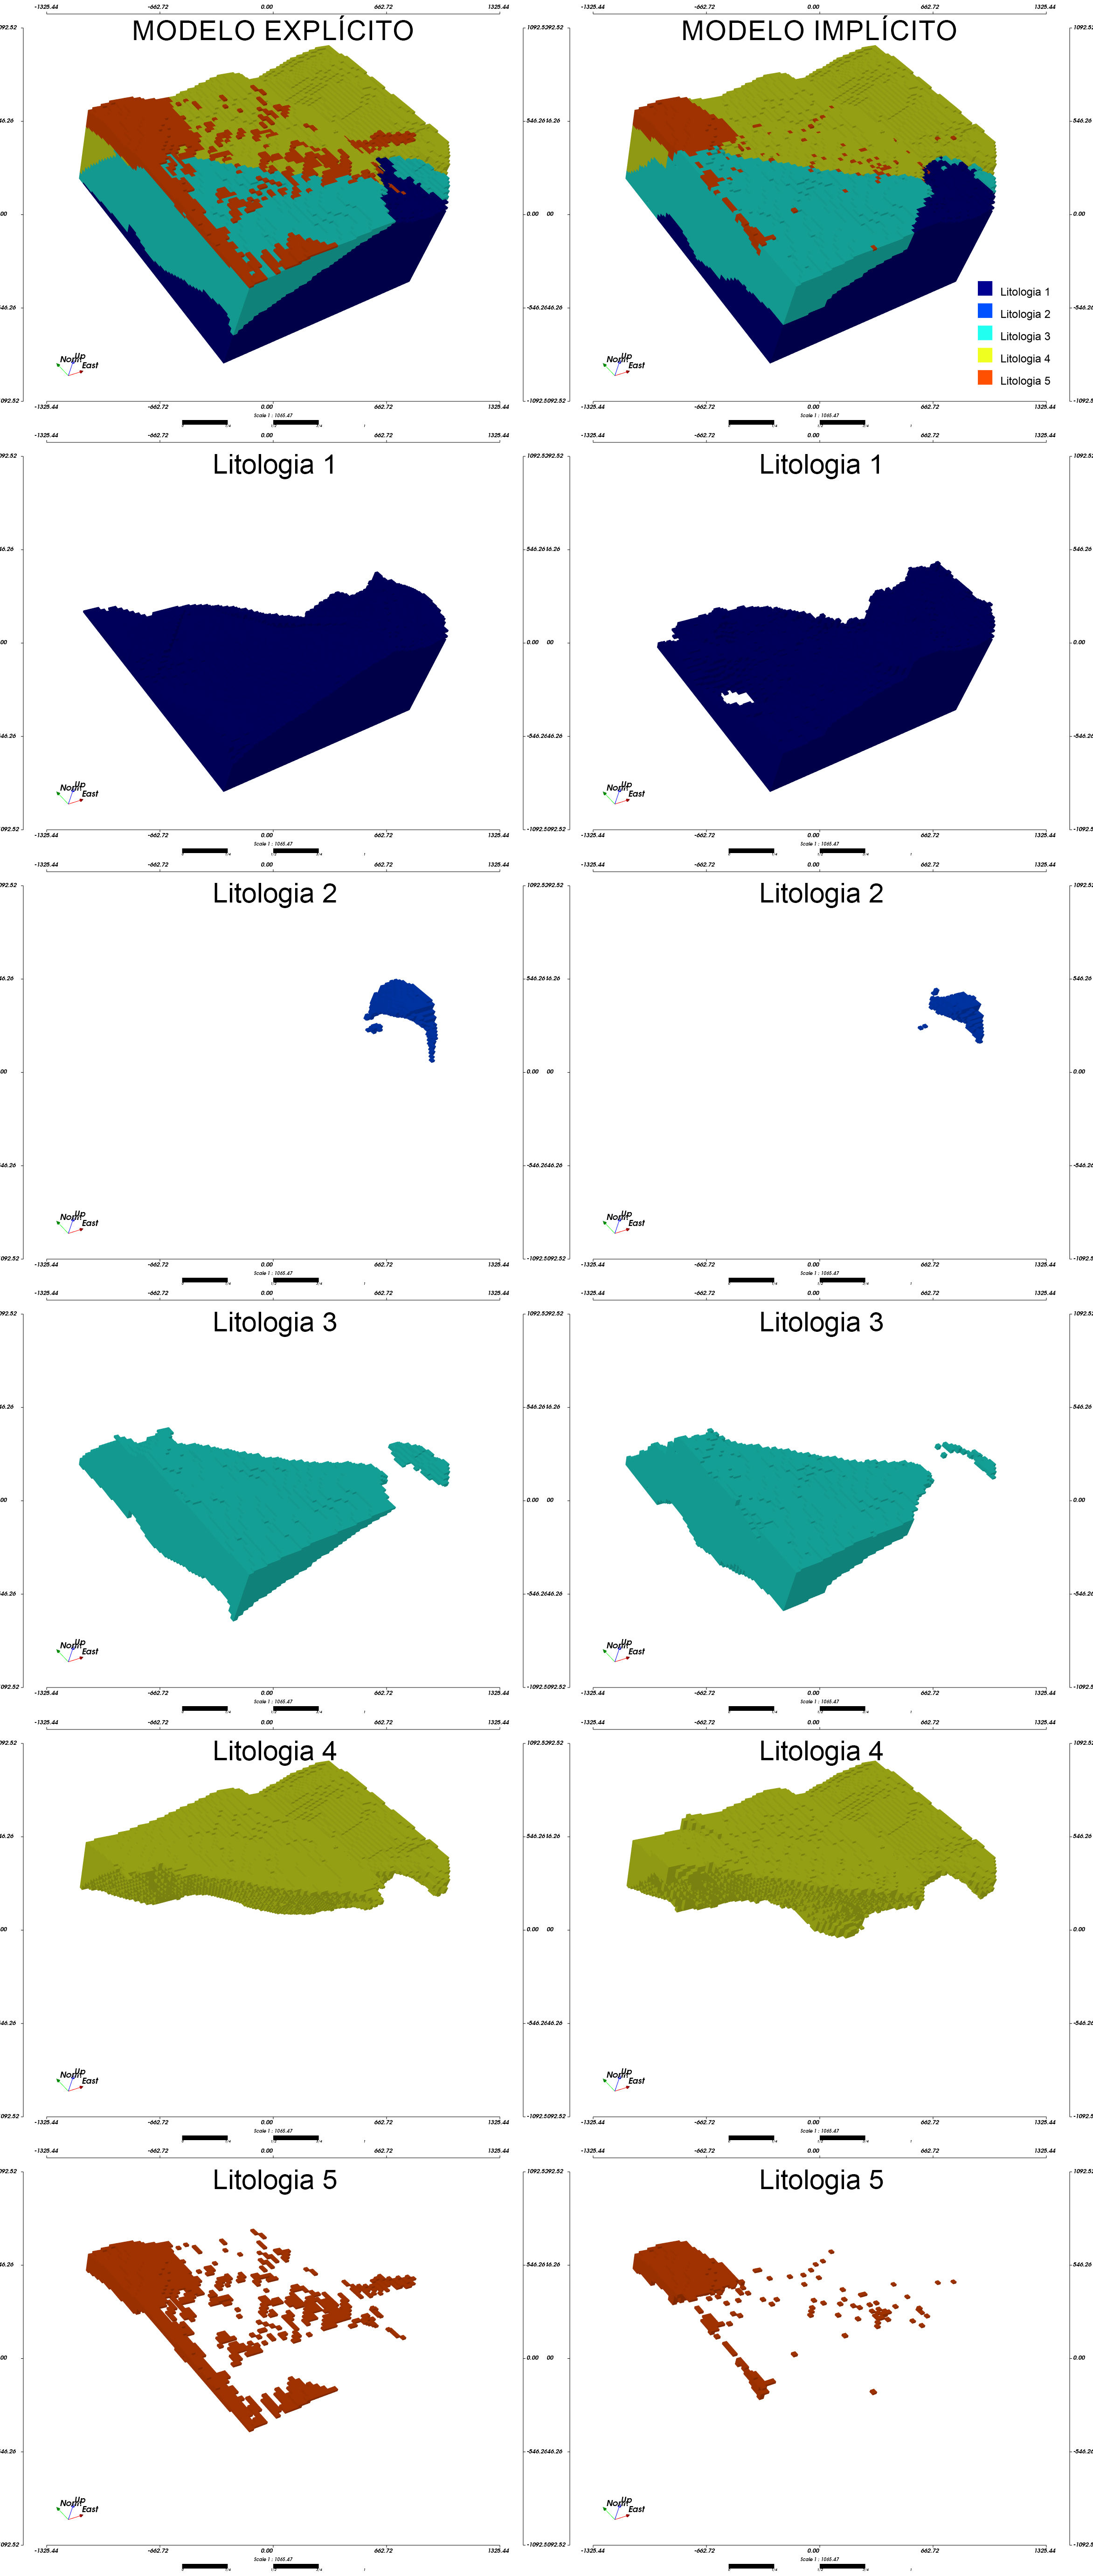
\includegraphics[width=0.65\textwidth]{estudo_de_caso/modelo3d}
	\end{center}
	%\legend{Fonte: Modificado de \citeonline{maureira}}
\end{figure}

A \autoref{scattermodelos} mostra o \textit{scatterplot} categórico entre os dois modelos criados: implícito no eixo y, e explícito no eixo x. Ao lado de cada ponto há o número de blocos comparados. Pontos que caem sobre a linha 45º são blocos concordantes em ambos os modelos, e pontos que caem fora dessa linha, blocos discordantes.

95\% dos blocos são concordantes em ambos os modelos. Todavia, apenas uma alta proporção de blocos concordantes não é indicativo de um bom modelo. Métodos menos sofisticados atingem alta proporção, 93\% no caso do vizinho mais próximo.   

\begin{figure}[H]
	\caption{\label{scattermodelos}\textit{Scatterplot} entre os modelos explícitos e implícitos.}
	\begin{center}
		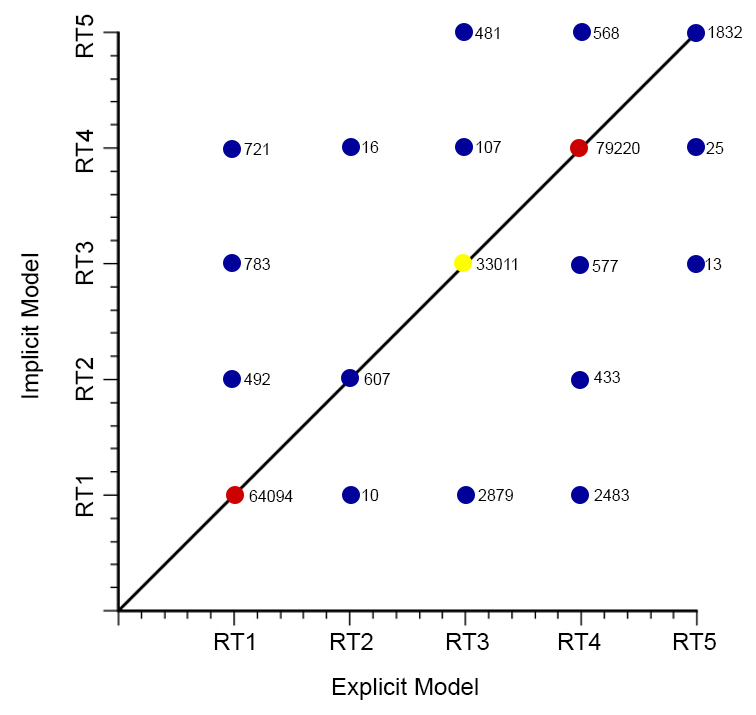
\includegraphics[width=0.7\textwidth]{estudo_de_caso/scatterplot_axis}
	\end{center}
	%\legend{Fonte: Modificado de \citeonline{maureira}}
\end{figure}

Porém, geram modelos que não fazem sentido físico do ponto de vista geológico, como observado na \autoref{nn}, um modelo gerado pela técnica do vizinho mais próximo a partir do mesmo banco de dados, são notáveis estruturas em forma de escada com mudança abrupta de angulação, diferentemente das formas suaves criadas pelo algoritmo proposto vistos na \autoref{modelo3d}.

\begin{figure}[H]
	\caption{\label{nn}Modelo criado utilizando a técnica do vizinho mais próximo.}
	\begin{center}
		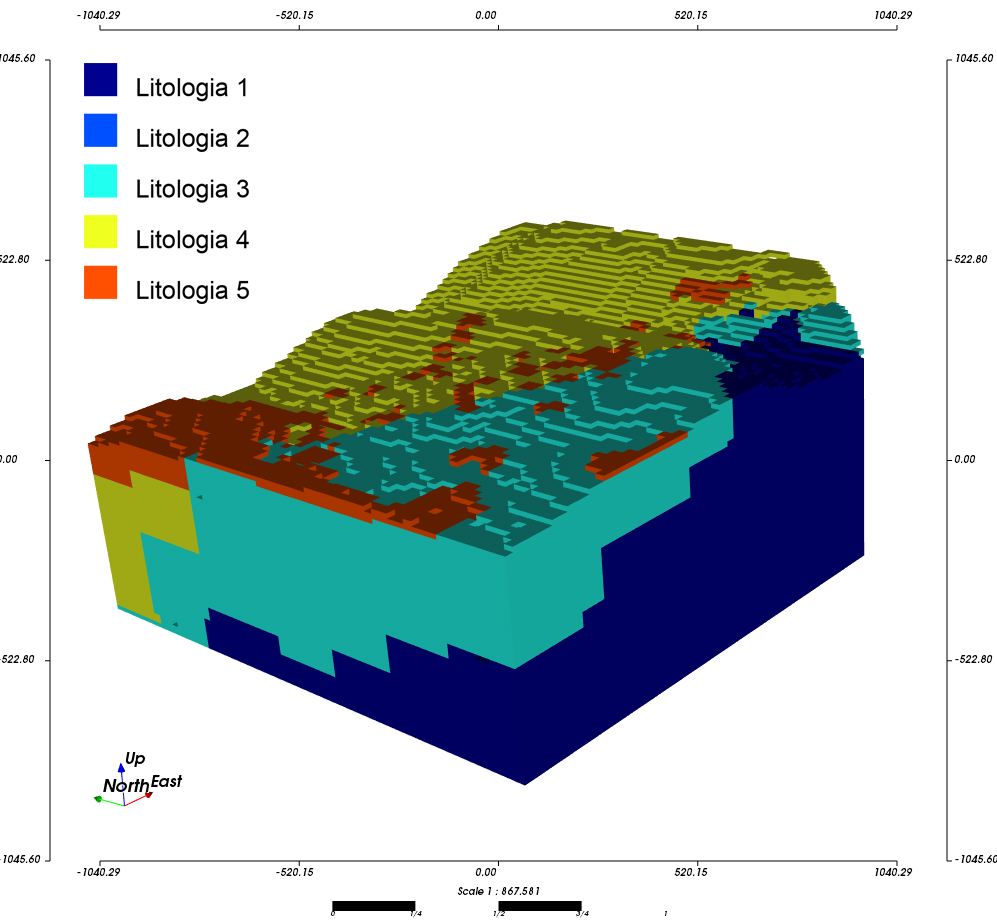
\includegraphics[width=0.6\textwidth]{estudo_de_caso/nn}
	\end{center}
	%\legend{Fonte: Modificado de \citeonline{maureira}}
\end{figure}

A incerteza também foi calculada como a probabilidade de cada de cada bloco pertencer a cada uma das categorias pela \textit{softmax transformation}. O parâmetro $\gamma=175$, valor padrão do \textit{plug-in}, foi escolhido. O resultado é mostrado nas seções verticais da \autoref{comparacao}.

\subsection{Comparação}\label{comparacao}

Uma comparação inicial pode ser feita observando os modelos, implícito e explícito, lado a lado na \autoref{modelo3d}. A litologia 5 aparece como blocos isolados e dispersos no modelo implícito, enquanto que no modelo explícito apresenta forma mais estruturada e contínua. Examinando a \autoref{dados}, percebe-se algumas amostras de litologia 5 espalhadas, em meio à abundantes amostras de outras litologias. O método das distâncias assinaladas não atribuirá aos blocos ao redor de amostras dispersas, sua litologia, já que a menor distância estimada para esses blocos será referente à categoria das amostras abundantes e agrupadas.

Os blocos isolados pertencentes à litologia 5 que aparecem no modelo implícito são blocos carimbados, após a geração do modelo baseado nas distâncias, com a litologia da amostra colocada, como visto no quadro Algoritmo 2 da \autoref{interpolator_sec}. O geomodelador aumentou a influência das amostras de litologia 5 no modelo explícito arbitrariamente ou munido de informação adicional, que não pode ser imputada no algoritmo proposto.

Para checar se o algoritmo reproduziu satisfatoriamente as estruturas interpretadas pelo geomodelador, seções verticais ao longo das direções x e y foram comparadas. Quatro seções espalhadas por toda extensão do modelo foram escolhidas em cada direção. 

Em x, o modelo apresenta 70 seções, a \autoref{secaox10} mostra a seção 10/70. À esquerda o modelo criado pelo geomodelador, ao centro o modelo criado pelo algoritmo proposto, à  direita blocos discordantes e concordantes e abaixo as probabilidades de cada bloco pertencer a cada uma das cinco categorias. Todas as seções analisadas seguem a mesma diagramação. 

Estruturas geológicas que foram reproduzidas satisfatoriamente pelo algoritmo foram destacadas por elipses verdes, enquanto estruturas que não foram bem reproduzidas, destacadas por elipses vermelhas.

Na região destacada pela elipse vermelha da \autoref{secaox10}, não há amostras da litologia 1. Provavelmente, o geomodelador munido de sua experiência e/ou informação adicional atribuiu a litologia 1 aos blocos dessa região. Note que alguns blocos na superfície do modelo implícito não foram carimbados com a litologia 5 como no modelo explícito. Porém, ao analisar a probabilidade RT5, existe uma chance considerável desses blocos pertencerem à litologia 5. mesmo que não tenham sido atribuídos àqueles blocos.   

\begin{figure}[H]
	\caption{\label{secaox10}Seção vertical 10/70 em x.}
	\begin{center}
		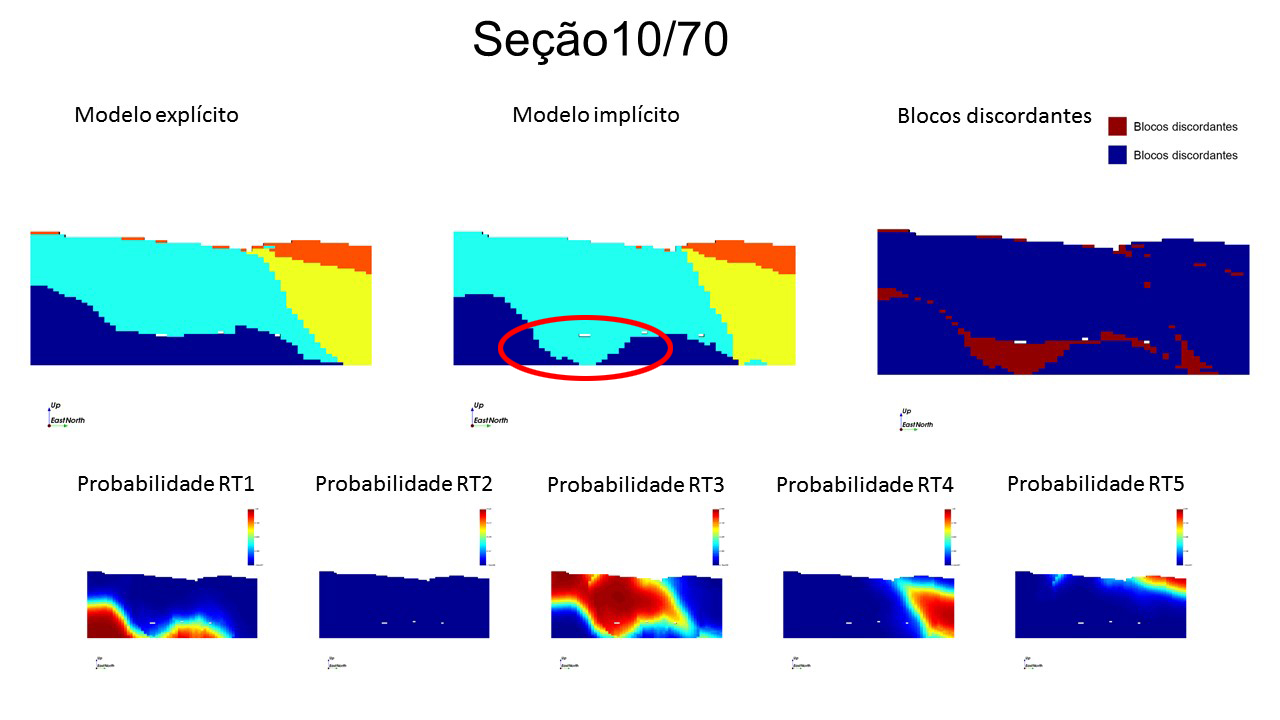
\includegraphics[width=0.9\textwidth]{estudo_de_caso/secaox10}
	\end{center}
	%\legend{Fonte: Modificado de \citeonline{maureira}}
\end{figure}

Na seção da \autoref{secaox37}, a região destacada pela elipse vermelha mostra uma estrutura desenhada pelo geomodelador no modelo explícito, com formas suaves e intricadas, de difícil reprodução pelos métodos matemáticos, a não ser em casos de alta densidade amostral. 

\begin{figure}[H]
	\caption{\label{secaox37}Seção vertical 37/70 em x.}
	\begin{center}
		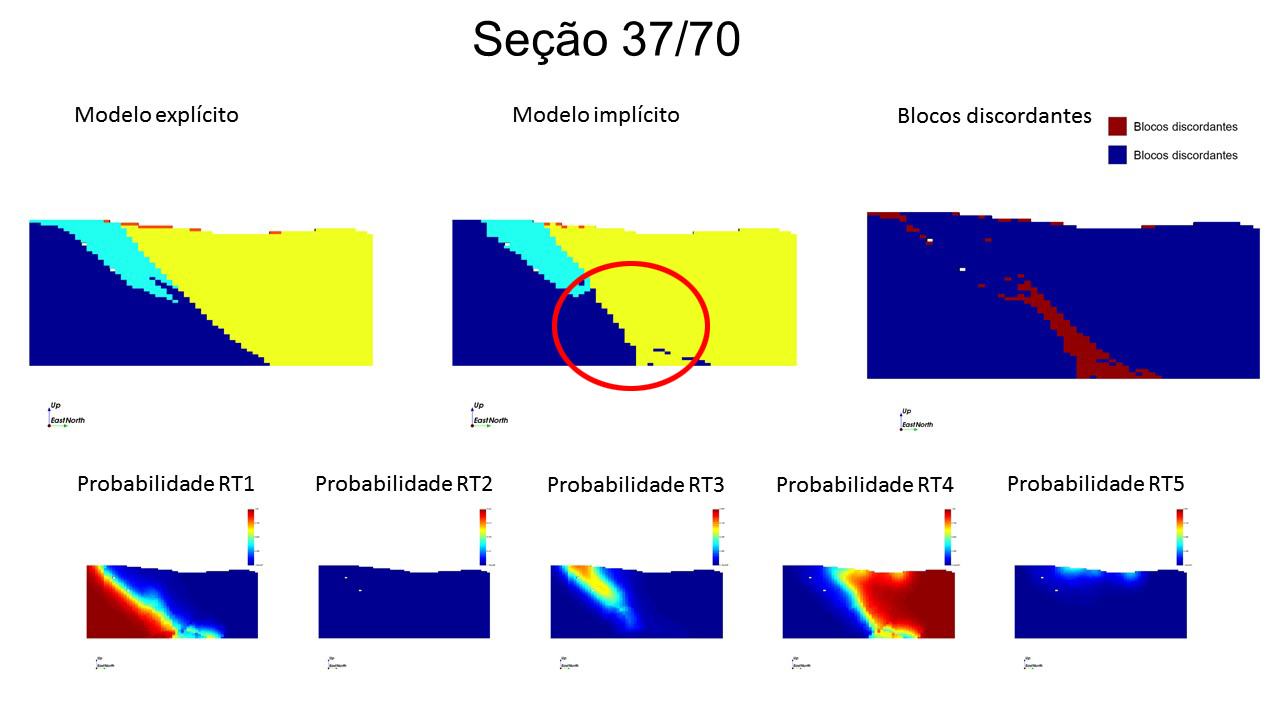
\includegraphics[width=0.9\textwidth]{estudo_de_caso/secaox37}
	\end{center}
	%\legend{Fonte: Modificado de \citeonline{maureira}}
\end{figure}

As estruturas presentes na seção 56 (\autoref{secaox56}), são estruturas pouco complexas, e foram bem reproduzidas pelo algoritmo.

\begin{figure}[H]
	\caption{\label{secaox56}Seção vertical 56/70 em x.}
	\begin{center}
		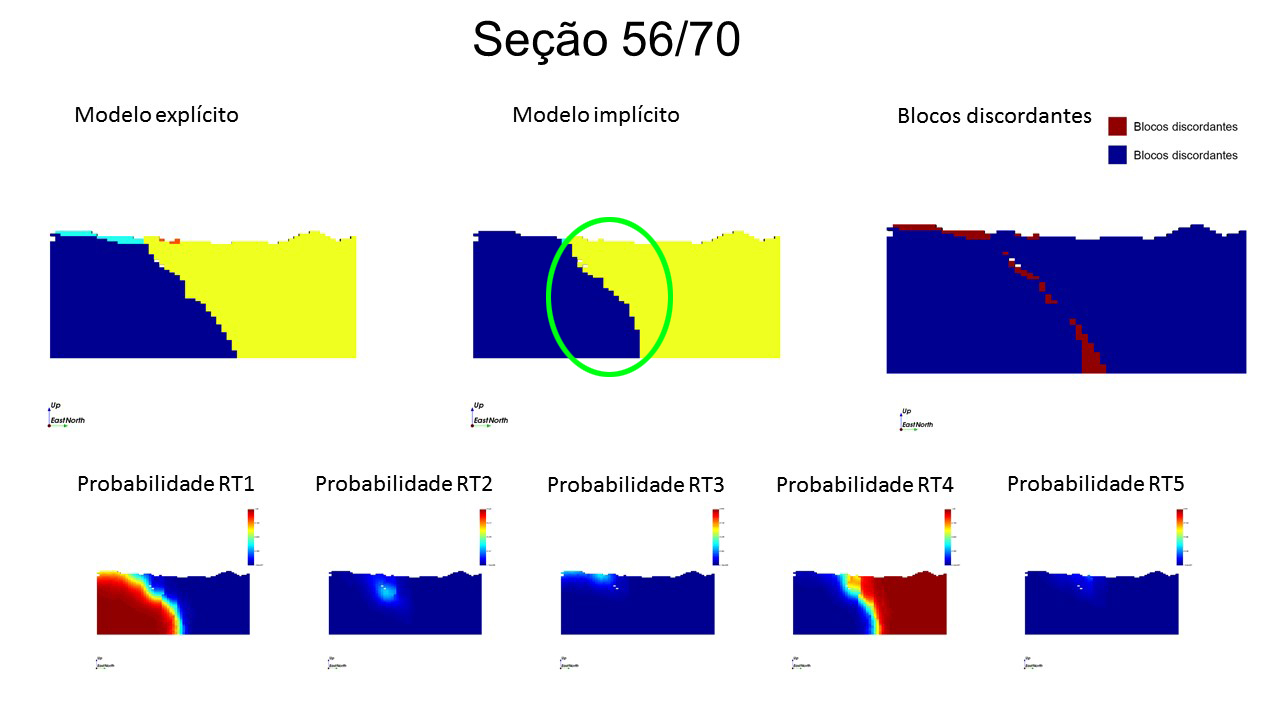
\includegraphics[width=0.9\textwidth]{estudo_de_caso/secaox56}
	\end{center}
	%\legend{Fonte: Modificado de \citeonline{maureira}}
\end{figure}

A seção da \autoref{secaox67}, mostra destacado pela elipse vermelha, uma estrutura que não foi bem reproduzida, o algoritmo deu mais volume à litogia 1 e menos à litologia 2 em relação ao modelo criado explicitamente. 

\begin{figure}[H]
	\caption{\label{secaox67}Seção vertical 67/70 em x.}
	\begin{center}
		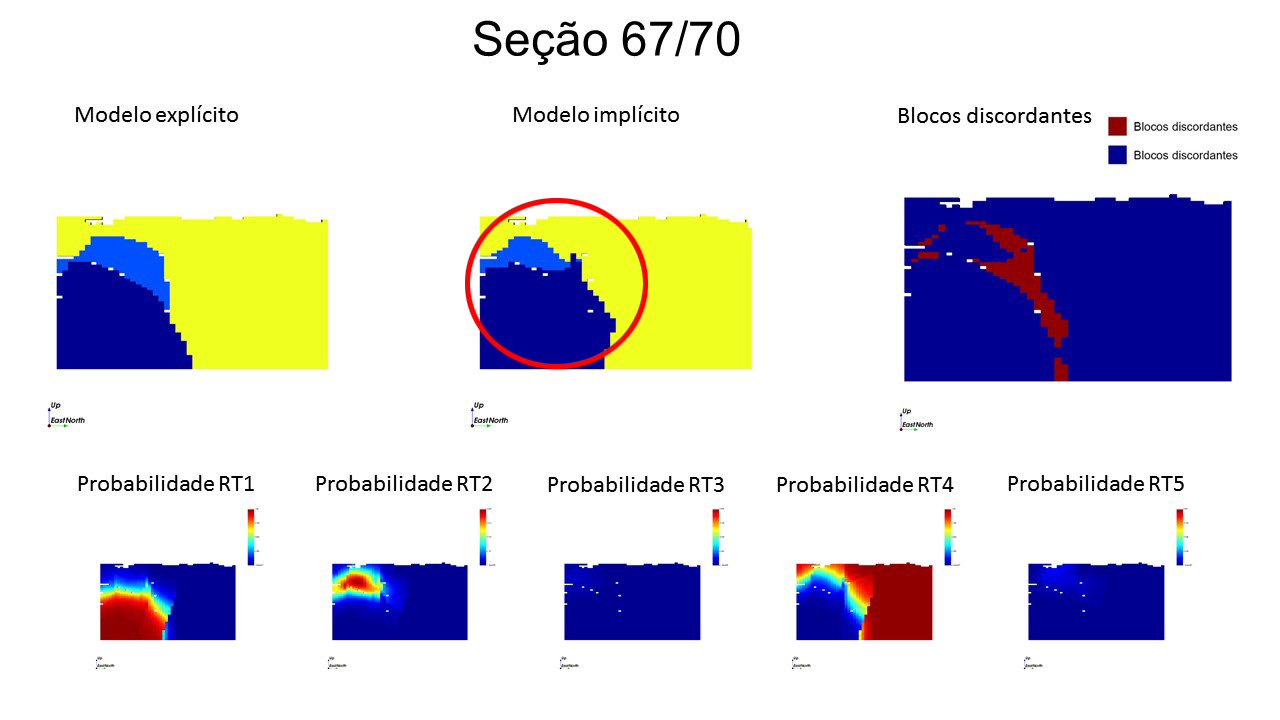
\includegraphics[width=0.9\textwidth]{estudo_de_caso/secaox67}
	\end{center}
	%\legend{Fonte: Modificado de \citeonline{maureira}}
\end{figure}

Na direção y, o modelo apresenta 60 seções. A seção 16 (\autoref{secaoy16}) exibe poucos blocos discordantes, o algoritmo reproduziu satisfatoriamente as estruturas interpretadas pelo geomodelador.

\begin{figure}[H]
	\caption{\label{secaoy16}Seção vertical 16/60 em y.}
	\begin{center}
		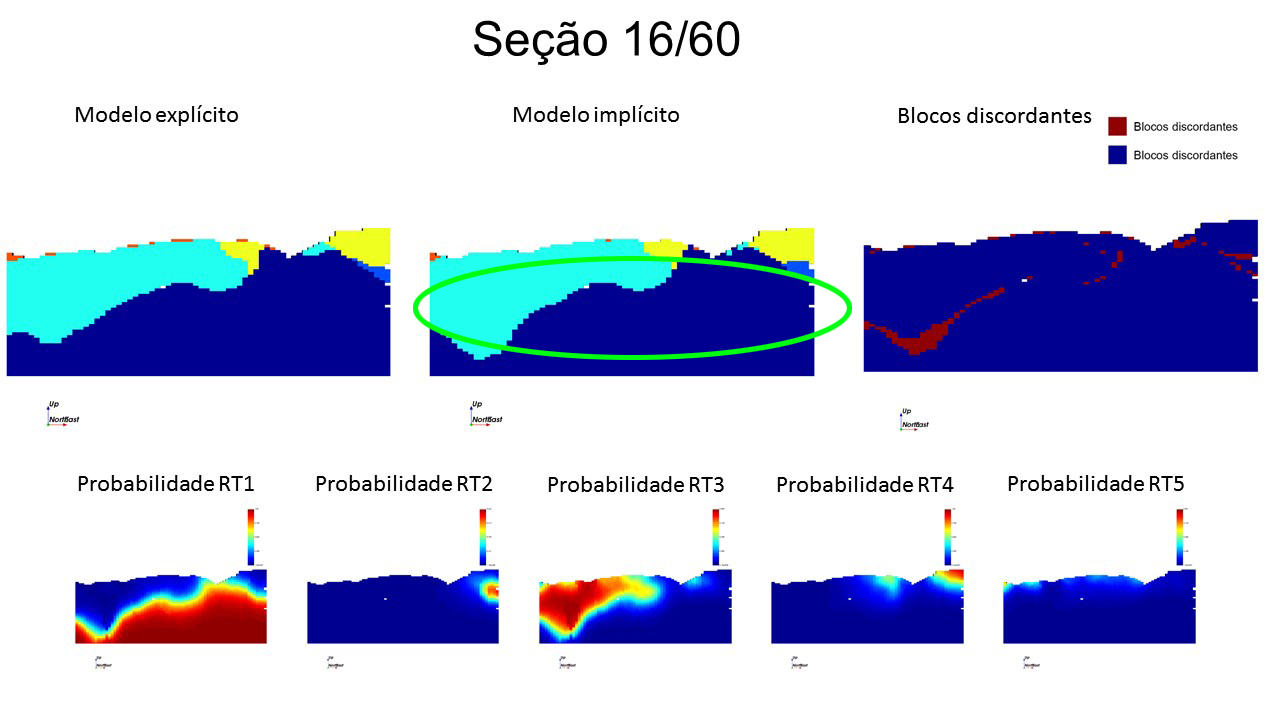
\includegraphics[width=0.9\textwidth]{estudo_de_caso/secaoy16}
	\end{center}
	%\legend{Fonte: Modificado de \citeonline{maureira}}
\end{figure}

Embora as estruturas interpretadas exibidas na \autoref{secaoy27} sejam bastante complexas, o algoritmo as reproduziu de forma razoável. 

\begin{figure}[H]
	\caption{\label{secaoy27}Seção vertical 27/60 em y.}
	\begin{center}
		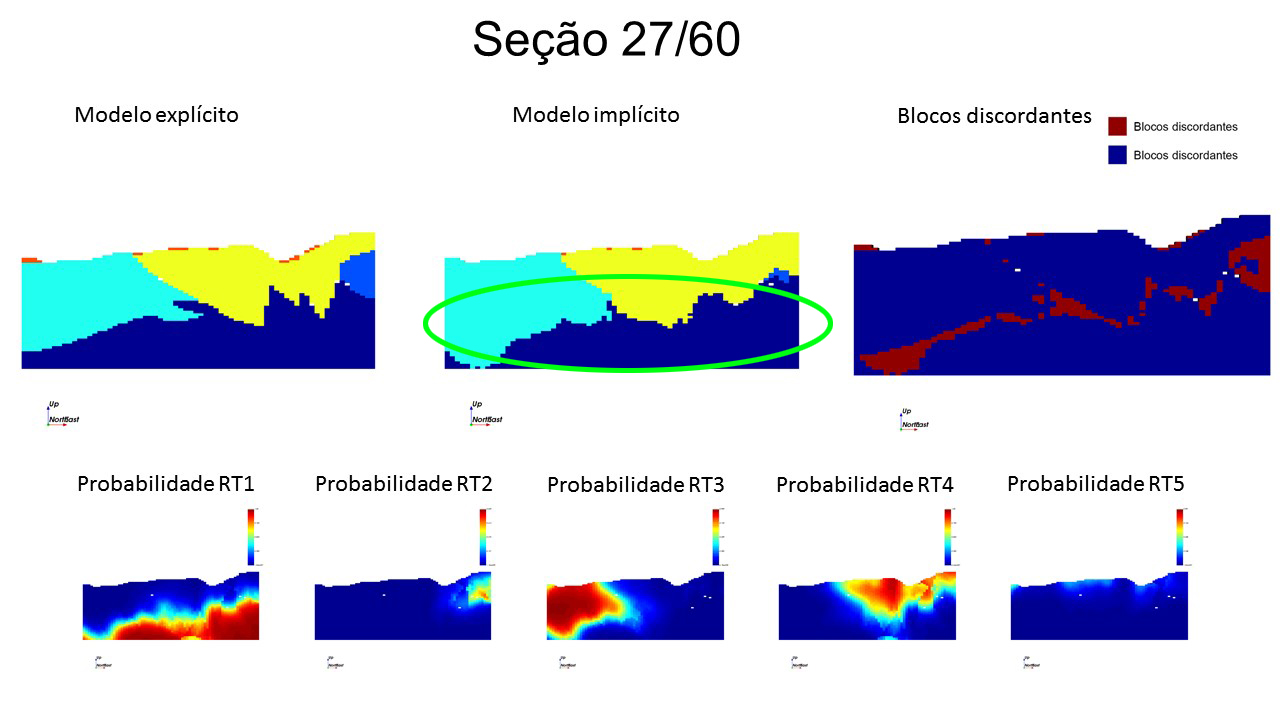
\includegraphics[width=0.9\textwidth]{estudo_de_caso/secaoy27}
	\end{center}
	%\legend{Fonte: Modificado de \citeonline{maureira}}
\end{figure}

Novamente, o método implícito reproduziu de forma satisfatória as estruturas interpretadas na \autoref{secaoy43}. 

\begin{figure}[H]
	\caption{\label{secaoy43}Seção vertical 43/60 em y.}
	\begin{center}
		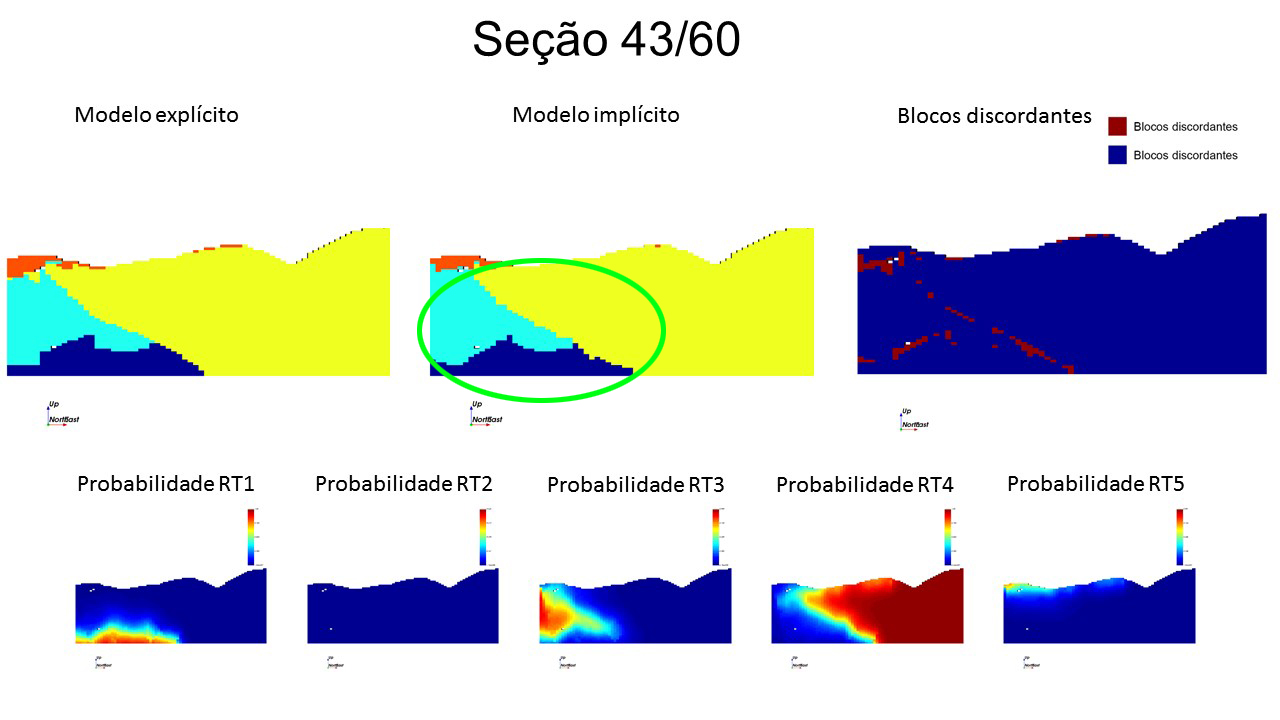
\includegraphics[width=0.9\textwidth]{estudo_de_caso/secaoy43}
	\end{center}
	%\legend{Fonte: Modificado de \citeonline{maureira}}
\end{figure}

A seção da \autoref{secaoy54} mostra, na zona destacada em vermelho, blocos atribuídos com a litologia 1 pelo geomodelador enquanto no modelo implícito esses blocos são atribuídos com a litologia 3. Novamente, essa é uma região sem amostras de litologia 1, o geomodelador, provavelmente, contou com sua experiência ou informação adicional para inferir a litologia desses blocos.

\begin{figure}[H]
	\caption{\label{secaoy54}Seção vertical 54/60 em y.}
	\begin{center}
		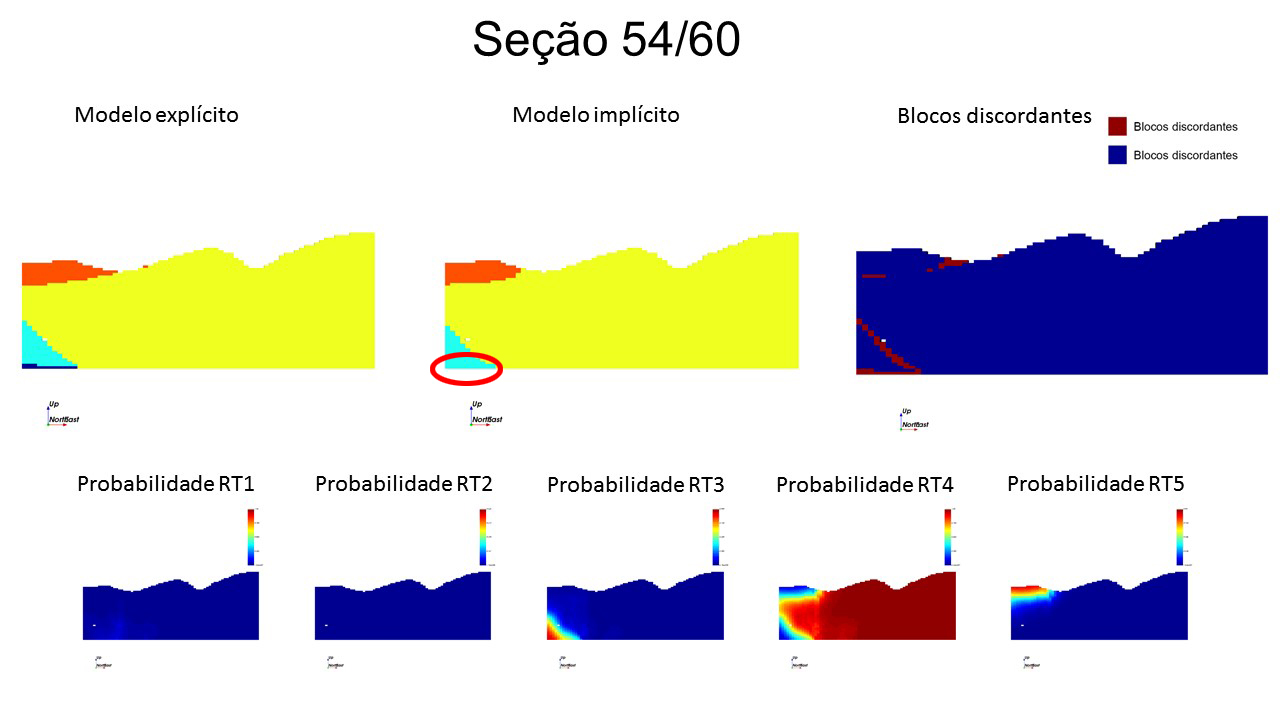
\includegraphics[width=0.9\textwidth]{estudo_de_caso/secaoy54}
	\end{center}
	%\legend{Fonte: Modificado de \citeonline{maureira}}
\end{figure}

Nesse estudo de caso, a aplicação do \textit{servo system} torna o modelo mais discordante em relação ao modelo de referência fornecido para comparação. Embora, as proporções dos dados ou dados desagrupados possam ser reproduzidas.

\section{Discussão}

A informação geológica é incorporada ao modelo através, não só do cálculo das distâncias assinaladas anisotrópicas, como também pelas direções de continuidade e efeito pepita dos variogramas. Limites suaves entre as litologias são garantidos pelo emprego da krigagem ordinária. Embora a complexidade geológica de pequena escala não seja bem reproduzida, devido ao efeito de suavização da krigagem, as grandes estruturas são bem representadas pelo algoritmo. A aplicação de um elipsoide de busca grande o suficiente e dados condicionantes em grandes quantidades aproximam os resultados da krigagem ordinária à krigagem global, evitando o surgimento de artefatos nos modelados gerados. O método implementado para múltiplos domínios geológicos evita sobreposição de litologias ou a necessidade de estabelecer qualquer tipo de ordem de prioridade para sua modelagem.

À primeira vista a modelagem dos variogramas para todas as categorias parece uma tarefa laboriosa e tediosa. Todavia, O comportamento contínuo das distâncias assinaladas os torna fáceis de modelar, e em muitos casos são semelhantes entre si, permitindo o uso de um mesmo modelo para todas as litologias. 

Algoritmos de modelagem geológica implícita devem satisfazer seis critérios estabelecidos por \citeonline{mclennan}: simplicidade, velocidade, objetividade, integração de dados, avaliação de incertezas e realismo geológico. O método proposto foi avaliado à luz desses critérios, a partir de observações feitas ao longo desse trabalho e do trabalho de \citeonline{maureira}. Pontos positivos e negativos são aqui apresentados.

\begin{itemize}
\item Simplicidade: O algoritmo é de simples implementação e não envolve nenhuma equação matemática complicada. A ideia de uma distância assinalada para cada domínio é de fácil compreensão;
\item Velocidade: O algoritmo é baseado em krigagem, que são métodos notadamente rápidos. A limitação é quanto ao número máximo de dados condicionantes usados na vizinhança de busca ao estimar cada bloco (acima de 200 tornam a execução bastante demorada);
\item Objetividade: A abordagem implícita surgiu para eliminar a subjetividade dos métodos explícitos de modelagem. É esperado que modelos sejam reproduzidos com exatidão quando os parâmetros envolvidos nos cálculos sejam os mesmos. Os modelos não estão sujeitos à influência individual de cada geomodelador;
\item Integração de dados: O algoritmo é flexível quanto à incorporação de novos dados do mesmo tipo. Entretanto, informação secundária (de outro tipo) não pode ser adicionada;
\item Avaliação de incerteza: O algoritmo não avalia incerteza baseado em múltiplas realizações equiprováveis de modelos geológicos. Contudo, uma forma alternativa de medição heurística da incerteza, baseada na transformação das distâncias estimadas em probabilidades, é implementada no método.
\item Realismo geológico: Modelos são considerados realísticos quando possuem concordância com a interpretação, e evidencias geológicas coletadas pelo geomodelador \cite{maureira}. A comparação da \autoref{comparacao}, mostra que o algoritmo reproduz satisfatoriamente, dadas suas limitações, as estruturas interpretadas. A krigagem ordinária, base do algoritmo, possui efeito de suavização. Então, embora estruturas de larga escala sejam bem reproduzidas, a reprodução da complexidade geológica de pequena escala fica comprometida.
\end{itemize}

Um geomodelador experiente dificilmente será substituído por um código e um computador. Porém, o algoritmo proposto é de grande ajuda, como método complementar à modelagem explícita. Principalmente, em fases iniciais do projeto ou na criação de proto modelos que devem ser refinados, poupando tempo e trabalho. À medida que a densidade amostral aumenta, o modelo implícito se torna mais próximo do modelo explícito.

Por fim, as vantagens e desvantagens da metodologia apresentada são discutidas.

Vantagens:

\begin{itemize}
\item Os modelos podem ser atualizados com facilidade e rapidez conforme novos dados são obtidos. Não há necessidade de nova digitalização manual;
\item Usando os mesmos parâmetros, os modelos são reproduzidos com exatidão, tornando a checagem e auditoria externa simples;
\item Uma variedade de análises de sensibilidade pode ser aplicadas ao modelo, variando parâmetros envolvidos na interpolação e nos variogramas das distâncias assinaladas;
\item O processo é rápido, poupando tempo e trabalho de geomodeladores na tediosa tarefa de construir e digitalizar manualmente seções verticais e horizontais.
\end{itemize}

Desvantagens:

\begin{itemize}
\item A interpolação das distâncias assinaladas pode impedir que um profissional treinado interprete estruturas e tendências da geologia que possam levar a melhores resultados;
\item O algoritmo é baseado em krigagem, então, apenas relações lineares entre domínios são modeladas (caso não existam amostras suficientes). A modelagem de estruturas complexas e curvilíneas depende de outros métodos geoestatísticos. Além disso, a propriedade suavizadora da krigagem compromete a modelagem da geologia de pequena escala;
\item O comportamento não estacionário das distâncias assinaladas torna a inferência do alcance dos variogramas arbitrária e questionável;
\item Não avalia incerteza baseado em múltiplas realizações equiprováveis do modelo;
\item O efeito de borda pode criar estruturas irreais nos limites do modelo.
\end{itemize}
